%% The first command in your LaTeX source must be the \documentclass command.
%%
%% Options:
%% twocolumn : Two column layout. Do not use twocolumn for papers submitted to CEUR-WS!
%% hf: enable header and footer.
\documentclass[
% twocolumn,
% hf,
]{ceurart}

%%
%% One can fix some overfulls
\sloppy

%%
%% Minted listings support
%% Need pygment <http://pygments.org/> <http://pypi.python.org/pypi/Pygments>
\usepackage{listings}
%% The Type1 Libertinus mono shipped with the class has proportional
%% capitals, which breaks the alignment of the SPARQL listings below.
\usepackage[varqu,varl]{zi4}
%% auto break lines
\lstset{breaklines=true, basicstyle=\ttfamily\footnotesize,
        columns=fullflexible, keepspaces=true, upquote=true}

%%
%% end of the preamble, start of the body of the document source.
\begin{document}

%%
%% Rights management information.
%% CC-BY is default license.
\copyrightyear{2026}
\copyrightclause{Copyright for this paper by its authors.
  Use permitted under Creative Commons License Attribution 4.0
  International (CC BY 4.0).}

%%
%% This command is for the conference information
\conference{Posters, Demos, Blue Sky, and Tutorials at SEMANTiCS 2026,
  Sep 2026, Ghent, Belgium}

%%
%% The "title" command
\title{Demonstration of RDF and SPARQL 1.2 Interoperability through
  Query Rewriting}

%%
%% The "author" command and its associated commands are used to define
%% the authors and their affiliations.
\author[1]{Jitse De Smet}[%
orcid=0009-0002-6513-5013,
email=jitse.desmet@ugent.be,
url=https://jitsedesmet.be/,
]
\author[2]{Maxime Jakubowski}[%
orcid=0000-0002-7420-1337,
email=maxime.jakubowski@tuwien.ac.at,
url=https://www.mjakubowski.info/,
]
\address[1]{IDLab, Department of Electronics and Information Systems,
  Ghent University -- imec, Belgium}
\address[2]{TU Wien, Austria}

%%
%% The abstract is a short summary of the work to be presented in the
%% article.
\begin{abstract}
  With the finalization of RDF 1.2 and SPARQL 1.2, the new triple-term
  construct brings native reification to RDF. Native support, however,
  does not imply uniform adoption: existing datasets continue to model
  statement-level metadata through established reification patterns,
  so federated queries must mediate between these patterns and the new
  syntax. We address this by rewriting queries written against triple
  terms into queries over the reification pattern actually used by
  each source, expressing the relationship as a SPARQL CONSTRUCT query
  that is unfolded into the user's query. This paper demonstrates the
  approach through a web interface in which users author their own
  mappings, select sources, and observe how their queries are
  rewritten and executed across federated endpoints.
  Reification translation is one application of a more general
  framework for SPARQL query answering under declarative RDF-to-RDF
  mappings, which we plan to formalize and optimize. The language gaps
  it exposes also give us concrete input for the upcoming SPARQL
  maintenance-mode standardization.\footnote{Video:
    \url{https://cloud.ilabt.imec.be/index.php/s/mm5ZipXsSkMDw5f}}
  \footnote{Canonical version:
    \url{https://2026-semantics-rewriting.jitsedesmet.be/}}
  \footnote{Demonstration:
    \url{https://2026-query-rewriting.demo.jitsedesmet.be/}}
\end{abstract}

%%
%% Keywords. The author(s) should pick words that accurately describe
%% the work being presented. Separate the keywords with commas.
\begin{keywords}
  SPARQL 1.2 \sep
  RDF 1.2 \sep
  Reification \sep
  Metadata \sep
  Data Integration \sep
  Query Rewriting
\end{keywords}

%%
%% This command processes the author and affiliation and title
%% information and builds the first part of the formatted document.
\maketitle

\section{Introduction}
\label{sec:introduction}

With the finalization of the recent RDF 1.2~\cite{rdf-1-2} and SPARQL
1.2~\cite{sparql-1-2} specifications, data publishers and consumers
will gain access to a newly introduced extension of the RDF data
model: the \emph{triple term}. This extension explicitly addresses the
need to have a uniform way of modelling statement-level metadata,
which previously was done with \emph{reification patterns}. Triple
terms enable arbitrary nesting of triples, bringing native reification
to RDF and narrowing the gap between RDF and Property
Graphs~\cite{iso-gql}. The construct directly descends from RDF-star
and SPARQL-star~\cite{hartig2017foundations}, proposed over a decade
ago.

However, standardization does not imply uniform adoption. Existing,
and even new, datasets might choose to continue modelling
statement-level metadata using established reification patterns (e.g.,
rdf-reification~\cite{spec:rdf-schema-1-1}, $n$-ary relations, or
potentially the vocabulary proposed in the draft RDF 1.2
interoperability note~\cite{spec:rdf-1-2-interop}). As a result,
querying RDF means handling all of these patterns, even though triple
terms now provide a single standard. The problem worsens in federated
settings, where sources may use different patterns, and the query
engine must mediate between them.

We address this gap with two contributions. First, we propose query
rewriting as a practical route to interoperability: SPARQL 1.2 queries
written against triple terms are rewritten into queries over the
reification pattern actually used by each source, with per-source
mappings handling federated heterogeneity. Second, we express these
mappings declaratively as standard SPARQL CONSTRUCT queries, keeping
the entire solution within the RDF ecosystem and requiring no new
mapping language. The rewriting algorithm itself builds on classic
unfolding techniques, applied to RDF 1.2.

The next section reviews related work on mapping and rewriting for
RDF. Section~\ref{sec:technique} describes our rewriting approach and
its limitations. Section~\ref{sec:demo} presents the demonstration,
and Section~\ref{sec:conclusion} concludes our paper.

\section{Related work}
\label{sec:related-work}

An imperative rewriting algorithm, such as the one proposed in the RDF
1.2 Interoperability note~\cite{spec:rdf-1-2-interop}, could handle a
fixed set of reification schemes. A declarative approach offers three
advantages over such an algorithm: 1. extensibility to reification
schemes not foreseen at design time, 2. interpretability of the
mappings themselves, and 3. reuse of existing SPARQL querying skills.
We therefore step back from an imperative algorithm and draw on the
data integration literature, where a Global-As-View (GAV) mapping
describes a global schema as a view over the local sources, and user
queries against the global are unfolded into queries over the
sources~\cite{lenzerini2002data}.

The closest prior work is POD-QUERY~\cite{pod-query}, which applies
GAV unfolding to RDF-to-RDF mappings. Each mapping rule names a single
\texttt{rml:source} paired with a query over it, expressed in
RML~\cite{rml}. Because RML rules are scoped to one source, POD-QUERY
inherits a single-source limitation: set-theoretic combinations across
sources $A$, $B$ and $C$, such as a global $D = (A \cup B) \setminus
C$, cannot be expressed as a single mapping. We instead write mappings
as SPARQL CONSTRUCT queries, which can federate across sources through
the SERVICE operator and so express such combinations directly.
Expressing mappings in SPARQL rather than RML also lowers the barrier
for RDF consumers, who typically know the former but not the latter.
POD-QUERY additionally predates RDF 1.2 and SPARQL 1.2, and so does
not address the triple-term rewriting that motivates this work.

A related line of work is Ontology-Based Data Access
(OBDA)~\cite{obda, obda-survey}, whose reference implementation is
Ontop~\cite{ontop}. OBDA also relies on GAV unfolding, but typically
maps relational sources --- through mapping languages such as
R2RML~\cite{spec:r2rml} --- to an ontology and layers
description-logic reasoning on top. When the sources are already RDF
and full TBox reasoning is not needed, plain GAV mediation is a
lighter-weight fit, and the SPARQL SERVICE operator provides the
federation across sources for free.

\section{Query rewriting}
\label{sec:technique}

Figure~\ref{fig:architecture} gives an overview of our approach: a
user query is sent to a federation mediator, which rewrites it through
one or more user-authored mappings into queries against the sources.
We express each mapping as a SPARQL CONSTRUCT query: the template
(mapping head) states what the mapping asserts about the global, and
the \texttt{WHERE} clause (mapping body) queries the source. When
several mappings target the same global, their outputs are implicitly
unioned, in line with RDF's dataset merge
operation~\cite{spec:rdf-semantics-1-2}. Figure~\ref{fig:mapping}
shows two such mappings: one constructs triple terms from
rdf-reification statements in the source, the other passes source
triples through unchanged. When a CONSTRUCT template contains multiple
triple patterns, we split it into one rule per triple pattern and
combine them through a \texttt{UNION} in the \texttt{WHERE} clause as
required by GAV-mapping theory; Figure~\ref{fig:mapping-as-one} shows
the equivalent single-headed form.

\begin{figure}
  \centering
  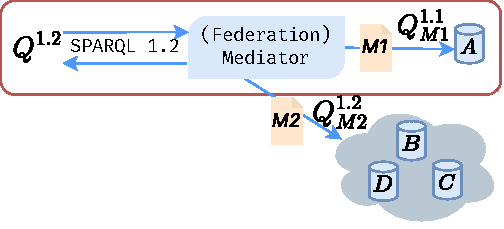
\includegraphics[width=0.8\linewidth]{interop}
  \caption{A SPARQL 1.2 query $Q^{1.2}$ enters the Federation
    Mediator, which rewrites it through user-authored mappings. The
    red box highlights the reification interoperability use-case:
    mapping $M1$ rewrites the query into $Q^{1.1}_{M1}$ against a
    single legacy source $A$ that uses an established reification
    pattern. The full figure depicts the general setting: $M2$ is a
    GAV mapping spanning multiple sources $B$, $C$, $D$, producing a
    federated query $Q^{1.2}_{M2}$. Each mapping is itself a SPARQL
    CONSTRUCT query; the mediator unfolds them into $Q^{1.2}$ and the
    rewritten query runs on any standards-compliant SPARQL 1.2
    federation engine.}
  \label{fig:architecture}
\end{figure}

\textbf{Algorithm.} The rewriting algorithm unfolds each triple
pattern in the user query against any mapping whose template (mapping
head) matches it, pushing additional constraints from the pattern into
the \texttt{WHERE} clause of the matching mapping. Consider the user
query in Figure~\ref{fig:user-query}, which asks for triple terms
whose inner predicate is \texttt{rdf:type} together with a confidence
score above \texttt{0.8}. The first triple pattern fixes the predicate
to \texttt{rdf:reifies} and the inner predicate of the triple term to
\texttt{rdf:type}; these constants flow into the unfolded body,
replacing \texttt{?p} by \texttt{rdf:type} in
Figure~\ref{fig:rewritten-query}. Mappings whose template cannot match
a pattern --- for instance because the predicates are incompatible ---
contribute a \texttt{FILTER(FALSE)} branch, which a downstream
optimizer can prune.

\begin{figure}[width=0.485\textwidth]
\begin{minipage}[t]{0.485\textwidth}
\begin{lstlisting}
# Create a mapping from rdf reification
# to triple terms
CONSTRUCT { ?t rdf:reifies <<( ?s ?p ?o )>> }
WHERE {
  ?t a rdf:Statement ; rdf:subject ?s ;
     rdf:predicate ?p ; rdf:object ?o ;
} # and copy all triples
CONSTRUCT { ?s ?p ?o } WHERE {
  ?s ?p ?o .
}
\end{lstlisting}
  \caption{Two mappings: one constructs triple terms in the global,
    the other passes source triples through unchanged.}
  \label{fig:mapping}
\end{minipage}\hfill
\begin{minipage}[t]{0.485\textwidth}
\begin{lstlisting}
CONSTRUCT { ?s ?p ?o } WHERE {
  { ?m_t a rdf:Statement ;
       rdf:subject ?m_s ;
       rdf:predicate ?m_p ;
       rdf:object ?m_o .
    BIND(?m_t as ?s) .
    BIND(rdf:reifies as ?p) .
    BIND(triple(?m_s, ?m_p, ?m_o) as ?o). }
  UNION
  { ?s ?p ?o }
}
\end{lstlisting}
  \caption{The same global as Figure~\ref{fig:mapping}, expressed as a
    single CONSTRUCT required for the GAV-unfolding algorithm.}
  \label{fig:mapping-as-one}
\end{minipage}
\end{figure}

\begin{figure}[width=0.485\textwidth]
\begin{minipage}[t]{0.485\textwidth}
\begin{lstlisting}
SELECT * WHERE {
  ?t rdf:reifies <<( ?s rdf:type ?o )>> ;
     ex:confidence ?score .
  FILTER(?score > 0.8)
}
\end{lstlisting}
  \caption{Example user query: triple terms asserting
    \texttt{rdf:type} with a confidence score above 0.8.}
  \label{fig:user-query}
\end{minipage}\hfill
\begin{minipage}[t]{0.485\textwidth}
\begin{lstlisting}
SELECT ?score ?o ?s ?t WHERE {
  { ?t rdf:type rdf:Statement ; rdf:subject ?s ;
       rdf:predicate rdf:type ; rdf:object ?o . }
  UNION { # Assume 1.1 sources ->
          # no triple terms
    FILTER ( FALSE ) }
  { # Predicate rdf:reifies does not
    # match ex:confidence
    FILTER ( FALSE ) }
  UNION { ?t ex:confidence ?score }
  FILTER ( ?score > 0.8 )
}
\end{lstlisting}
  \caption{Cleaned-up version (for readability) of the query in
    Figure~\ref{fig:user-query} rewritten against the mapping in
    Figure~\ref{fig:mapping-as-one}. The rewritten query no longer
    asks the source for triple terms; instead it expresses the same
    intent through the reification scheme used by the source.}
  \label{fig:rewritten-query}
\end{minipage}
\end{figure}

\textbf{Scope.} Although this paper focuses on RDF 1.2
interoperability, the rewriting framework is more general: we envision
it as a broader approach to SPARQL query answering under mappings, of
which reification-pattern translation is one application. Because the
rewritten query is itself a federated SPARQL query, the approach
inherits the boundaries of federated SPARQL. Blank nodes have limited
support on both sides of a mapping: CONSTRUCT templates and the
\texttt{BNODE} expression introduce fresh blank nodes scoped to a
single query solution, and blank nodes returned by a source cannot be
matched across invocations of the same endpoint, since blank nodes are
scoped to the document or result set in which they are
serialized~\cite{sparql-1-2}. Skolemization is the classical solution.
Recursive property paths (\texttt{*} and \texttt{+}) are likewise not
handled, pending a recursive extension to SPARQL.

\section{Demonstration}
\label{sec:demo}

The demo's main scenario is RDF 1.2 interoperability: the user writes
a SPARQL 1.2 query using triple terms, points it at one or more
sources that model statement-level metadata through legacy reification
patterns, and sees the query rewritten so that it runs against the
sources as-is. The rewritten query is shown next to the original, so
users can inspect how it was transformed using
Traqula~\cite{traqula}, and then executed using
Comunica~\cite{comunica}. Alongside this main scenario, the demo ships
with several preset scenarios that exercise different facets of the
framework: 1. wikidata reification, 2. exhaustive source selection,
3. uniprot reification, and 4. paper filter Verborgh.

In the Wikidata reification example, we construct the global by
copying all existing triples and adding triple terms to statements
following Wikidata's $n$-ary reification approach; we then query the
\emph{instance of} property of Belgium. The exhaustive source
selection example runs over the RDF profiles of Bryan, Ruben, and
Jitse, querying the names of all scholarly articles on their profiles.
The UniProt example again copies all existing triples and adds triple
terms, this time following the standard RDF reification that UniProt
uses; we then query the annotations of a given protein. Finally, the
set-theoretic example shows how these combinations work in practice:
we construct the global as every triple in Jitse's and Ruben's
profiles, except those related to articles that Verborgh also
describes. Querying the scholarly articles and their names in this
global, we see that Jitse's vision paper is missing, for instance,
because Verborgh co-authored it.

The query rewriting mechanism is not limited to reification
translation. Any mapping the user writes becomes part of the global
schema, and the rewriting handles it identically. Federation across
sources is itself a special case: selecting a set of endpoints is
equivalent to a second layer of GAV rewriting in which every mapping
has the form
\texttt{CONSTRUCT \{ ?s ?p ?o \} WHERE \{ SERVICE <s> \{ ?s ?p ?o \} \}},
which the engine performs as exhaustive source
selection~\cite{heterogeneous_fedqpl}. The demo thus stands in for a
broader claim from Section~\ref{sec:technique}: that mapping-driven
query rewriting is a general way to query RDF under user-defined
schemas, with reification interoperability as one application.

The interface exposes this through four panels. The \emph{mappings
  panel} (top left) is where the user writes CONSTRUCT queries that
together define the global schema. The \emph{query panel} (top right)
is where the user selects sources and writes the user query against
that schema. The \emph{rewritten query panel} (bottom left) is
read-only and shows the user query unfolded against the mappings after
execution. The \emph{results panel} (bottom right) reports elapsed
execution time, the result count, and the streaming bindings as they
arrive.

\begin{figure}
  \centering
  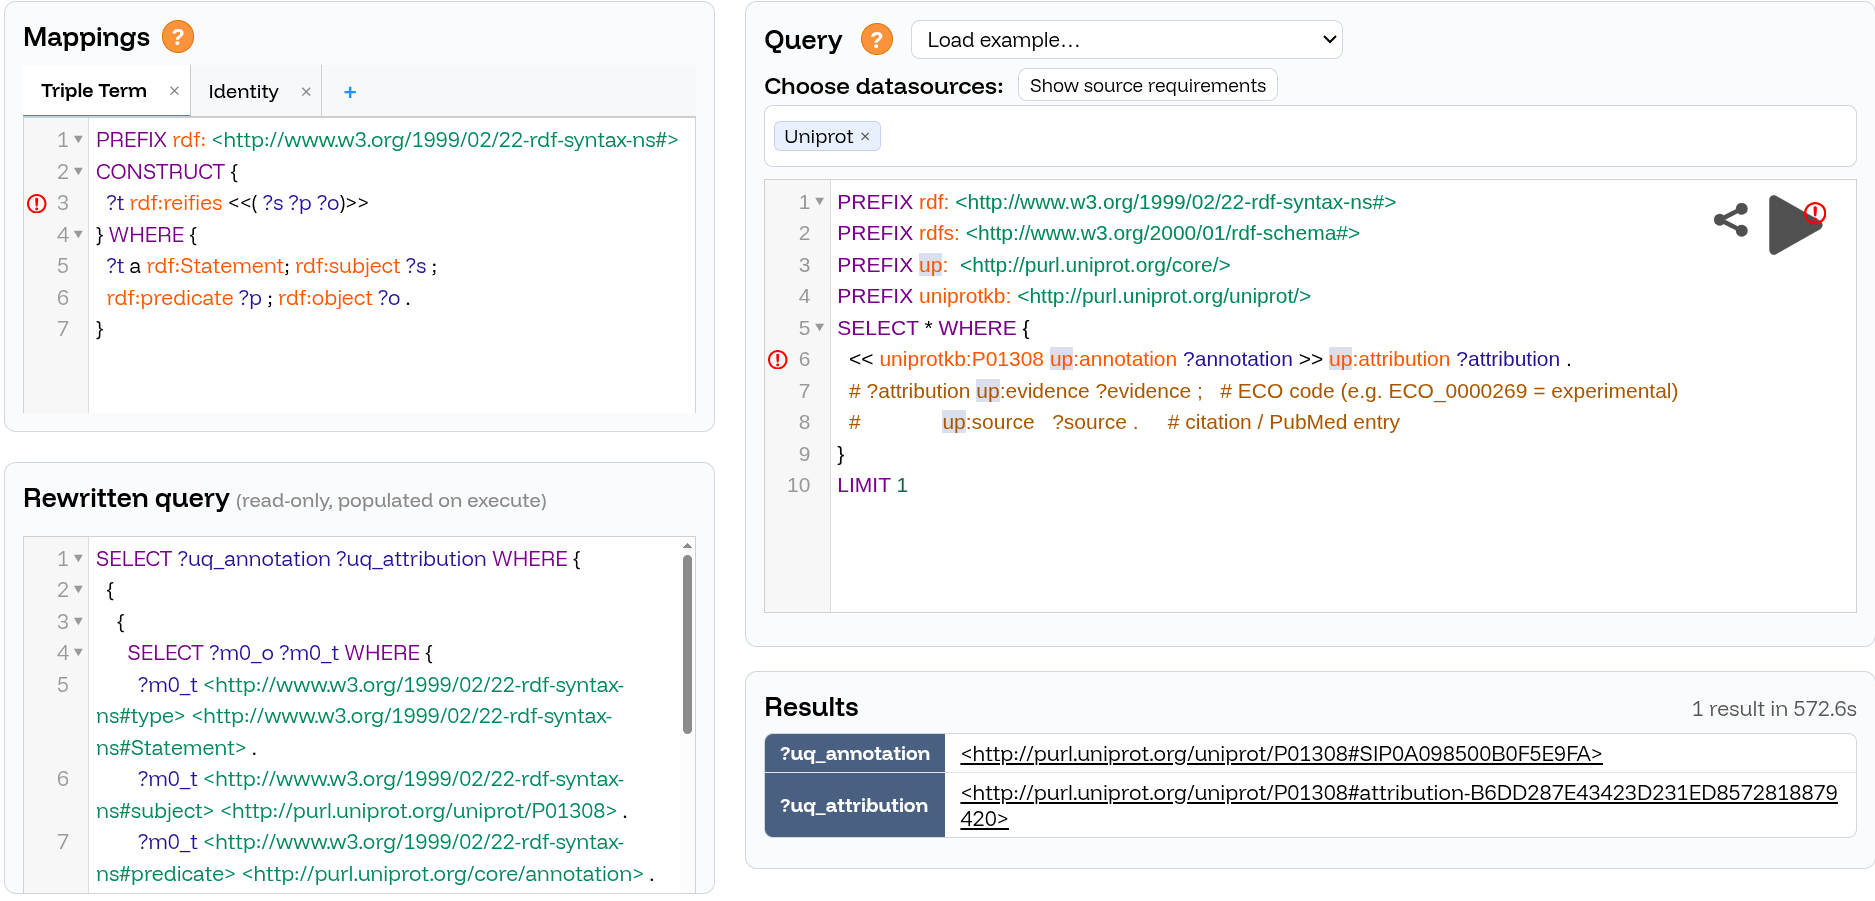
\includegraphics[width=0.75\linewidth]{screenshot}
  \caption{Screenshot of the web interface: a user query is rewritten
    against user-defined mappings and executed over the chosen
    sources.}
  \label{fig:screenshot}
\end{figure}

\section{Conclusion}
\label{sec:conclusion}

We have presented a preliminary implementation of query rewriting for
RDF 1.2 interoperability, addressing the gap between the new
triple-term construct and the reification patterns that datasets
continue to use in practice. This use-case is one instantiation of a
more general vision: SPARQL query answering over declarative
RDF-to-RDF mappings, of which reification translation is one
application among many.

The mappings are GAV rules expressed as SPARQL CONSTRUCT queries, and
rewriting proceeds by unfolding those rules into the user's query.
This declarative approach buys three things over a handwritten
algorithm: 1. extensibility to reification schemes not foreseen at
design time; 2. interpretable transformations that users can read
directly; and 3. reuse of existing SPARQL skills, since mappings are
written in the same language as the queries they rewrite. Because both the rules and the rewriting live within SPARQL, the
rewritten query runs on any standards-compliant SPARQL 1.2 federation
engine, with no engine modification required.

This is ongoing work. Immediate next steps include performance
optimization, and broader applications beyond reification translation.
A separate thread is concrete input to the upcoming maintenance-mode
standardization of SPARQL: when a desired mapping cannot be expressed
in standard SPARQL, the missing feature becomes a candidate language
extension. We have already encountered a handful: a \texttt{CONSTRUCT
  GRAPH} form, syntactic sugar for triple-term templates, and
recursive view definitions. Our aim with this demonstration is to draw
attention to GAV-style SPARQL mappings, to showcase their use for RDF
1.2 interoperability, and to open discussion on the language features
the community needs to make the broader vision practical.

%%
%% The acknowledgments section is defined using the "acknowledgments" environment
%% (and NOT an unnumbered section). This ensures the proper
%% identification of the section in the article metadata, and the
%% consistent spelling of the heading.
\begin{acknowledgments}
  This publication is based upon work from COST Action CA23147
  GOBLIN---Global Network on Large-Scale, Cross-domain and
  Multilingual Open Knowledge Graphs, supported by COST (European
  Cooperation in Science and Technology). Jitse De Smet is a
  predoctoral fellow of the Research Foundation - Flanders (FWO)
  (1SB8525N).
\end{acknowledgments}

%% The declaration on generative AI comes in effect
%% in Janary 2025. See also
%% https://ceur-ws.org/GenAI/Policy.html
\section*{Declaration on Generative AI}

During the preparation of this work, the author(s) used Claude Opus
4.7 in order to: Paraphrase and reword, improve writing style, perform
grammar and spelling checks, and critically review the text written by
the authors to highlight essential information. After using these
tool(s)/service(s), the author(s) reviewed and edited the content as
needed and take(s) full responsibility for the publication's content.

%%
%% Define the bibliography file to be used
\bibliography{references}

\end{document}

%%
%% End of file
